%% -*- coding:utf-8 -*-
\author{Stefan Müller}\institute[HU Berlin, Institut für deutsche Sprache und Linguistik, Syntax]{}

\settowidth\jamwidth{(Niederländisch)}

\subtitle{Phenomena}

\section{Phenomena}

\huberlintitlepage[22pt]

\outline{

\begin{itemize}
%\item {Überblick über die germanischen Sprachen}
\item \alert{Phenomena}
\item Phrase structure grammars and \xbart
\item Valence, order of arguments and adjuncts
\item Verb clusters in SOV langauges
\item Verbposition: Verb first and verb second order
\item Passive
%\item embedded sentences
\end{itemize}

}



% \frame{
% \frametitle{Übungsaufgaben/Wiederholung}


% Bestimmen Sie in den folgenden Sätzen die topologischen Felder, die Wortarten der Wörter, die Kasus der Nominalgruppen und die
% grammatischen Funktionen und zeichnen Sie für einen Satz einen Strukturbaum in einem theoretischen
% Modell Ihrer Wahl (\zb Government \& Binding)!
% \eal
% \ex Der Mann lacht.
% \ex Der Frau hat der Mann das Buch gegeben, den wir kennen.
% \ex Ein Lied singend ging Peter voran.
% \ex Einen Aufsatz schreiben, der komplett neue Gedanken enthält,\\
%     können nur wenige.
% \zl

% }

\frame{
\frametitle{Introductory material}


Terminology (part of speech, grammatical functions, topological fields, \ldots): Chapter~1 in \citew{MuellerGT-Eng}.
\begin{refsection}

\nocite{MuellerGT-Eng}

\printbibliography[heading=none,notkeyword=this]

\end{refsection}

\pause

Overview of phenomena: Chapter~2 in \citew{MuellerGermanic}.


\begin{refsection}

\nocite{MuellerGermanic}

\printbibliography[heading=none,notkeyword=this]

\end{refsection}





}


  


\frame{
\frametitle{Variation}

\begin{itemize}
\item order:
\begin{itemize}
\item VO vs.\ OV
\item V2 vs. Non-V2
\item order of subjects and objects (fixed or free)
\item order of adverbs
\end{itemize}
\item verb clusters
\item subject requirement
\item passive
\begin{itemize}
\item personal passive
\item impersonal passive
\item objects of ditransitive verbs
\end{itemize}
\item expletives
\begin{itemize}
\item marking of clause type in main clauses (V2)
\item marking of clause type in embedded clauses (V3)
\end{itemize}
\end{itemize}


}


\subsection{Warning: OV/VO vs.\ V2/non-V2}

\frame{
\frametitle{Warning: OV/VO vs.\ V2/non-V2}


\begin{itemize}
\item Languages are classified according to order of subject, object and verb:
\begin{itemize}
\item SOV
\item SVO
\item \ldots
\end{itemize}
\item This does not mean that all sentences of a language always correspond to this pattern.
\item Languages are classified according to their type.

\item independent property: V2 or not V2.

\item third independent property:\\
      possibility to reorder subject and objects (Scrambling).

\item \citet{Haftka96a}:\\
      \emph{Deutsch ist eine V/2-Sprache mit Verbendstellung und freier Wortfolge}

German is a V2 language with verb in final position and free constituent order.

Sounds crazy, but it is not.

\end{itemize}
}


\subsection{Order of subject, object and verb}

\frame[shrink]{
\frametitle{Order of subject, object \& verb in the world's languages}

\medskip

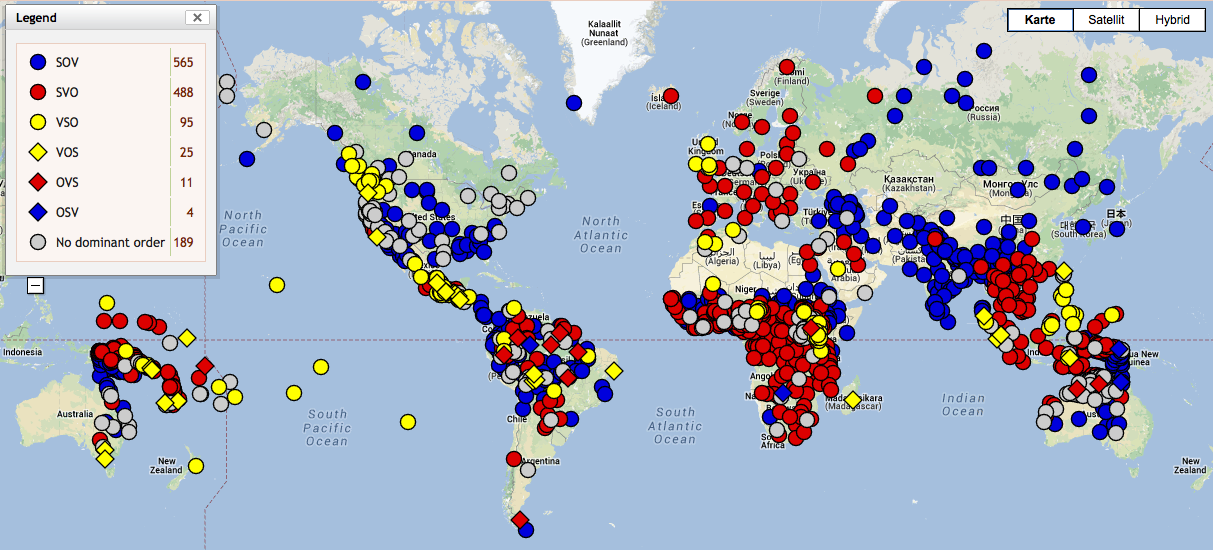
\includegraphics[width=\textwidth]{Bilder/WALS-SOV}

\vfill

{\small Matthew S. Dryer: Feature 81A: Order of Subject, Object and Verb,\\
 The World Atlas of Language Structures} 


}

\frame{
\frametitle{Subject, object and verb in the WALS}


\pause
\begin{itemize}
\item Subjects are arguments with more agent-like properties.
\pause
\item Objects are arguments with more patient-like properties.
\pause
\item This is not necessarily what we assume to be subjects and objects within traditional grammars
  of particular languages.\\ For example German: Subject = nominative \citep{Reis82}
\ea
\gll Der Aufsatz interessiert mich.\\
     the paper   interests    me\\
\glt `I am interested in the paper.'
\z
\end{itemize}



}

\frame{
\frametitle{Dryer: Word order}

\begin{itemize}
\item Dryer: Determining Dominant Word Order

\emph{Where a language is shown on one of the word order maps as having a particular order as the dominant
order in the language, this means that it is either \blaubf{the only order possible} or the order
that is \blaubf{more frequently used}.


I base my classification of Macushi here on the frequency counts, and since no order is more than
twice as frequent as the next most frequent order, I treat this language as lacking a dominant order
of subject, object, and verb.}

\bigskip

German, Dutch and Frisian are V2 languages, that is, SVO and SVAuxOV orders are the result of verb
fronting with a semantic function. These languages are usually counted among the SOV languages as well.

\end{itemize}



}

\frame{
\frametitle{Subject, object, verb in Europe}

\begin{columns}[T]
\begin{column}{90mm}
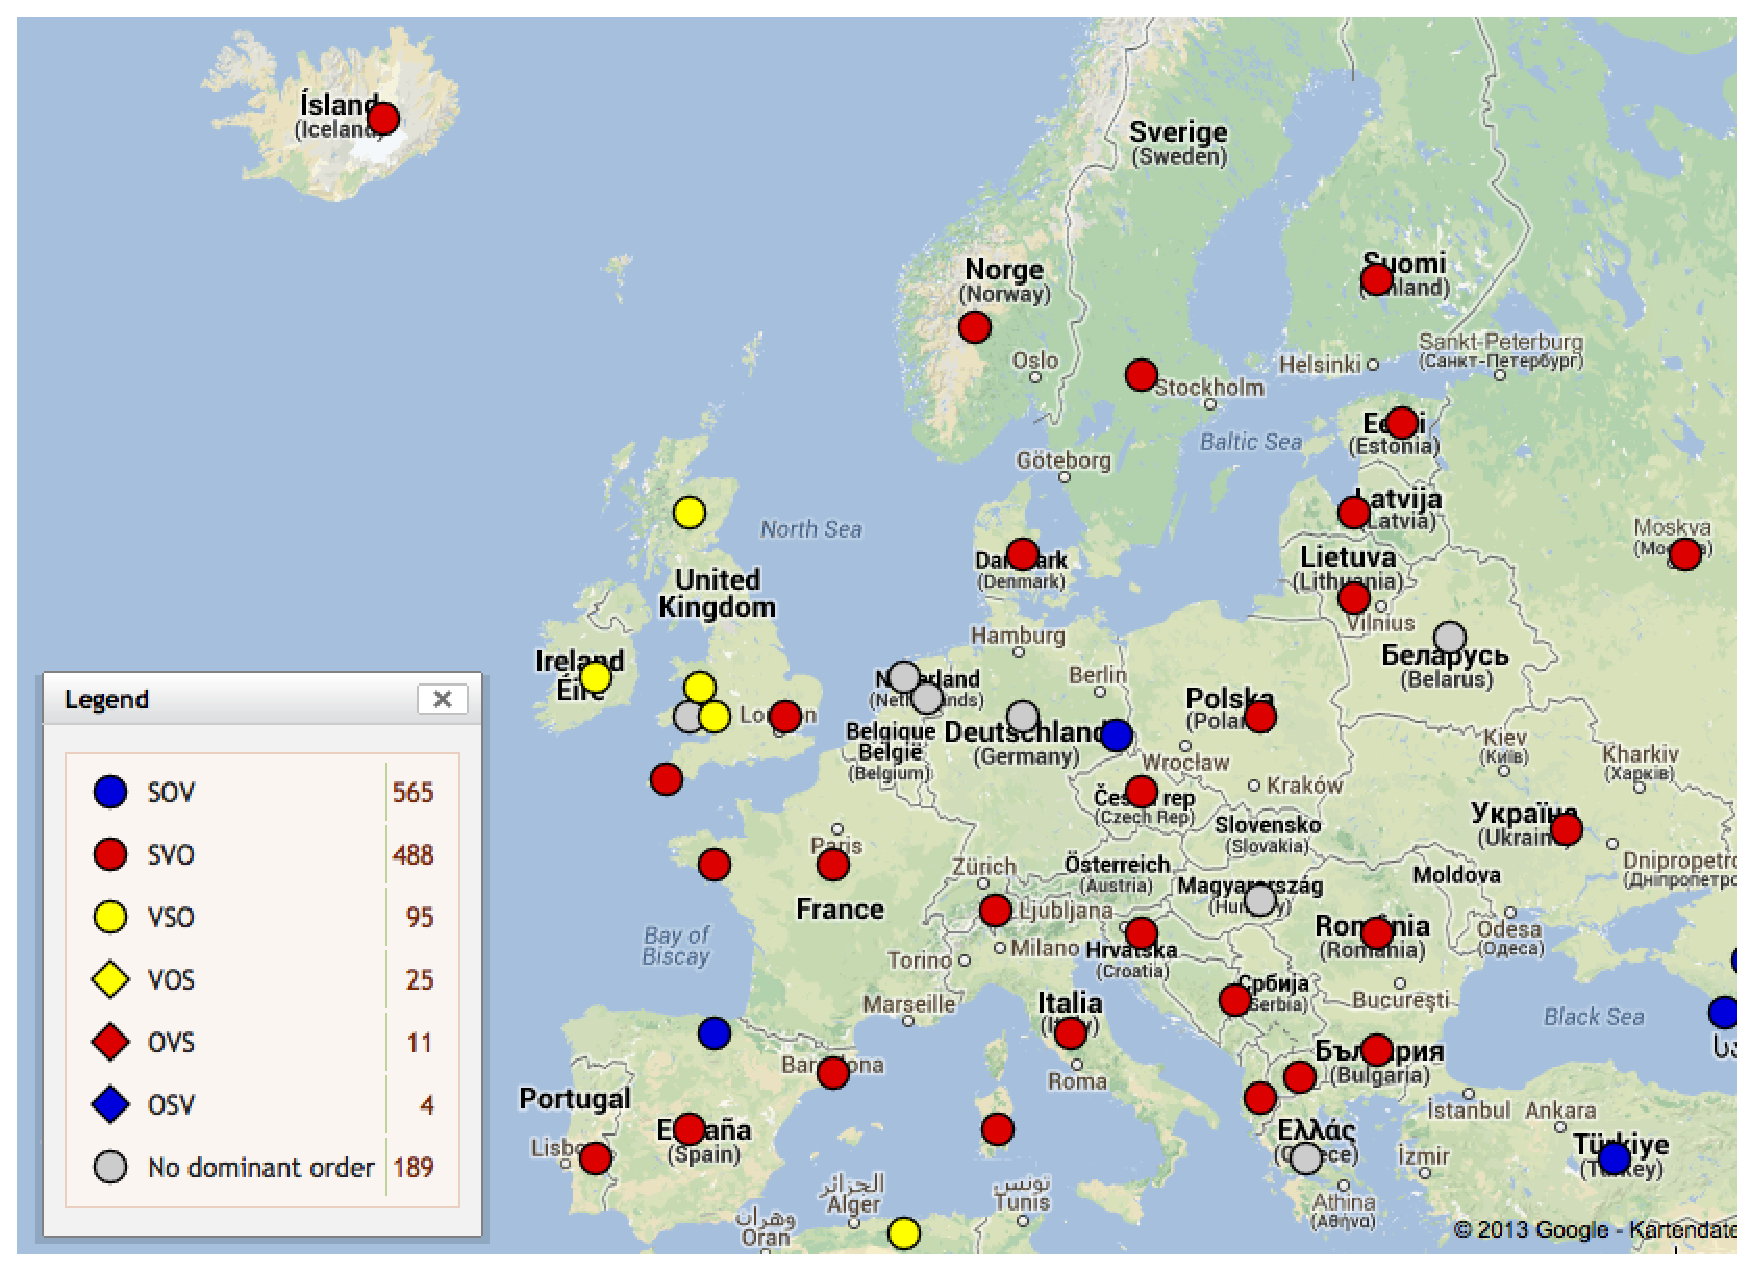
\includegraphics[width=\textwidth]{Bilder/WALS-SOV-Europa}
\end{column}
\begin{column}{25mm}
SVO:\\
Islandic,\\
Norwegian,\\
Swedish,\\
Danish,\\
English
\end{column}
\end{columns}
}


\frame{
\frametitlefit{Dryer: Feature 81b: Two Dominant Orders of Subject, Object, and Verb}

\begin{columns}[T]
\begin{column}{90mm}
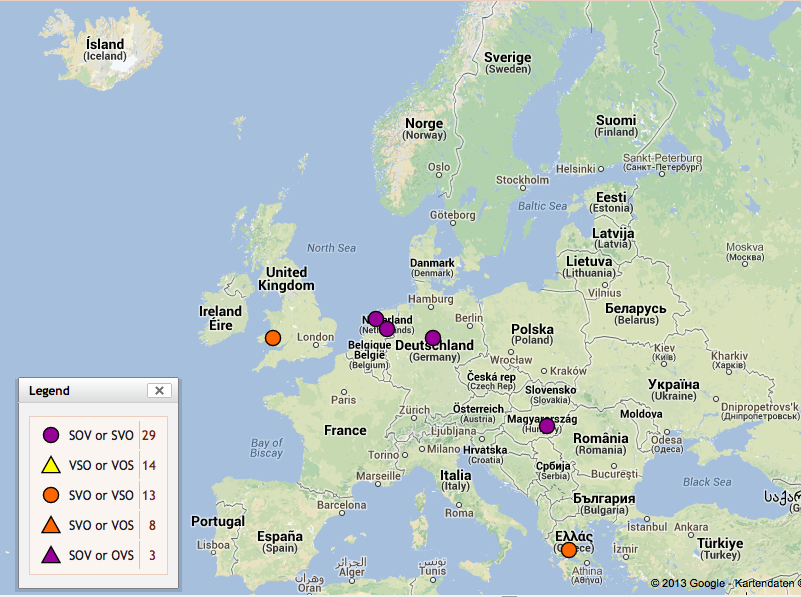
\includegraphics[width=.95\textwidth]{Bilder/WALS-SOV-Europa-no-dominant}
\end{column}
\begin{column}{30mm}
SVO oder SOV:\\
German,\\
Frisian,\\
Dutch
\end{column}
\end{columns}
% Walisisch: SVO oder VOS
% Friesisch
% Niederländisch
% Deutsch 
% Ungarisch

}
% Eisenberg89:409 zitiert Greenberg66 mit Deutsch als SVO.


\frame{
\frametitle{Languages without a dominant order in the WALS}

Dryer:

A third subtype of language lacking a dominant order consists of languages in which different word
orders occur but the choice is syntactically determined. For example, in \blaubf{German and Dutch}, the
dominant order is \blaubf{SVO in main clauses lacking an auxiliary} and \blaubf{SOV in subordinate clauses and
clauses containing an auxiliary} [\ldots]. Because this results in both orders being
common, neither order is considered dominant here and these two languages are shown on the map as
lacking a dominant word order. In general, if the word order varies according to whether there is an
auxiliary verb, the language is shown on the map as lacking a dominant order.


}

\frame{
\frametitle{Auxiliaries do not count, or do they?}

\eal
\ex 
\gll Kim sieht den Fuchs.\\
     Kim sees the fox\\
\glt `Kim sees the fox.'
\ex
\gll Kim hat den Fuchs gesehen.\\
     Kim has the fox seen\\
\glt `Kim has seen the fox.'
\zl
Dreyer classifies (\mex{0}a) as SVO and (\mex{0}b) as SAuxOV.\\
Aux is ignored so that the pattern counts as SOV.
\pause

}

\frame{
\frametitle{Other verb embedding verbs?}

But what about (\mex{1})?
\eal
\ex 
\gll Kim scheint den Fuchs zu sehen.\\
     Kim seems   the fox  to see\\ \hfill(SVOV?)
\glt `Kim seems to see the fox.'

\pause

\ex 
\gll Kim scheint den Fuchs gesehen zu haben.\\
     Kim seems   the fox  seen to have\\
\glt `Kim seems to have seen the fox.'
\zl

It is just the finite verb that is placed differently because of clause type marking.

}

\frame{
\frametitle{OV vs.\ VO: OV}

OV: Verbs follow the object:

\eal
\ex
\gll dass sie ihn sieht$_1$\\
     that she him sees\\\jambox{(German, SOV)}
\glt `that she sees him'
\ex
\gll dass sie ihn gesehen$_2$ hat$_1$\\
     that she him seen        has\\
\glt `that she has seen him'
\ex
\gll dass sie ihn gesehen$_3$ haben$_2$ muss$_1$\\
     that she him seen        have     must\\
\glt `that she must have seen him'
\zl

Embedding verbs follow embedded ones.

}

\frame{
\frametitle{OV vs.\ VO: VO}

VO: Verbs precede their object:

\eal
\ex
\gll at   hun ser$_1$ ham\\
     that she  sees    him\\\jambox{(\ili{Danish, SVO})}
\ex
\gll at   hun have$_1$ set$_2$ ham\\
     that she  has      seen    him\\
\ex
\gll at   hun må$_1$ have$_2$ set$_3$ ham\\
     that she  must   have     seen   him\\
\zl

OV: German, Dutch, Afrikaans, \ldots

VO: English, Danish, Norwegian, Swedish, \ldots

}

\frame{
\frametitle{Particle verbs and resultative constructions}

%[Section~15.2]
\citet{Haider2020a}: further differences between VO and OV languages:

Particle verbs:
\eal
\ex Kim will \alert{look up} the information.      \hfill(verb < particle)
\ex Kim wird die Information \alert{nachschlagen}. \hfill(particle < verb)
\zl
\pause

Resultative constructions:
\eal
\ex Kim will \alert{fish} the pond \alert{empty}.       \hfill(verb < pred)
\ex Kim wird den Teich \alert{leer} \alert{fischen}.    \hfill(pred < verb)
\zl

}

\subsection{V2}

\frame{
\frametitle{V2}

\begin{itemize}
\item German (and other Germanic languages) are V2 languages:\\
      The finite verb is in second position in assertions and \emph{w} questions.
\item An arbitrary constituent can be placed in front of it:
\eal
\ex 
\gll Das Kind  gibt dem Eichhörnchen jetzt eine Nuss.\\
     the child gives the squirrel now a nut\\\jambox{(\ili{German})}
\glt `The child gives the squirrel a nut now.'
\ex 
\gll Dem Eichhörnchen gibt das Kind jetzt eine Nuss.\\
     the squirrel gives the child now a nut\\
\ex 
\gll Eine Nuss gibt das Kind dem Eichhörnchen jetzt.\\
     a nut gives the child the squirrel now\\
\ex 
\gll Jetzt gibt das Kind dem Eichhörnchen eine Nuss.\\
     now gives the child the squirrel a nut\\
\zl
% \eal
% \ex 
% \gll Wer gibt dem Eichhörnchen jetzt eine Nuss?\\  
%      who gives the squirrel now a nut\\\jambox{(\ili{German})}
% \glt `Who gives the squirrel a nut now?'
% \ex 
% \gll Wem gibt das Kind jetzt eine Nuss?\\
%      who gives the child now a nut\\
% \glt `Who does the child give a nut to now?'
% \ex 
% \gll Was gibt das Kind dem Eichhörnchen jetzt?\\
%      what gives the child the squirrel now\\
% \glt `What does the child give the squirrel now?'
% \ex 
% \gll Wann gibt das Kind dem Eichhörnchen eine Nuss?\\
%      when gives the child the squirrel a nut\\
% \glt `When does the child give the squirrel a nut?'
% \zl
\end{itemize}

}

\frame{
\frametitle{V2 vs.\ non-V2}

\begin{itemize}
\item All Germanic languages are V2, except English:
\eal
\ex Bagels mag ich.\jambox{(German)}
\ex Bagels, I like.\jambox{(English)}
\zl 


\eal
\ex Gestern gab ich dem Eichhörnchen eine Nuss.\jambox{(German)}
\ex Yesterday, I gave the squirrel a nut.\jambox{(English)}
\zl 

\item There is fronting in English, but the fronted constituent is placed\\ before the subject and the
  verb.

\end{itemize}

}

\frame{
\frametitle{Non-extractable Elements}

Allmost all arguments can be frotned in V2 langauges.

Not all objects may be fronted in English (speaker dependent) \citep[\page 258]{Hudson92a-u}:

\eal
\judgewidth{\%}
\ex[]{
We give children sweets.
}
\ex[]{
These sweets, we give children \_.
}
\ex[\%]{
These children, we give \_ sweets.
}
\zl

}

\frame{
\frametitle{Fronting may cross clause boundaries}



\ea
\gll [Über dieses Thema]$_i$ habe ich sie gebeten, [[einen Vortrag \_$_i$~] zu halten].\footnotemark\\
     \spacebr{}about this topic  have I her asked \hphantom{[[}a talk {} to hold\\\german
\footnotetext{
Adapted from \citew[\page 21]{HN89b}.
}
\glt `I asked her to give a talk about this topic.'
\z

This means that V2 cannot be local reordering of constituents.


}


\frame{
\frametitle{V2 and OV/VO}

\begin{itemize}
\item V2 is independent of VO/OV. Danish is SVO and V2.
\eal
\ex 
\gll Gert har læst bogen.\\
     Gert has read book.\textsc{def}\\\danish
\ex
\gll Bogen har Gert læst.\\
     book.\textsc{def} has Gert read\\
\zl


\end{itemize}

}

\frame{
\frametitle{Englisch as Residual V2}

There is a residuum of V2 structures in questions:
\eal
\ex Which book did Sandy read?
\ex Which book did Sandy give to Kim?
\ex To whom did Sandy give the book?
\zl

\citet[\page 375]{Rizzi1990a-u}:  \emph{residual V2 language}


}


\frame{
\frametitle{Clause types}

Clause types are encoded via verb position. Apart from assertions and interrogative \emph{w}
clauses, there are V2 imperatives:

\ea
\gll Jetzt gib ihr das Buch!\\
     now give her the book\\\german
\glt `Give her the book now!'
\z
\pause

Yes/no questions and imperatives as V1:
\eal
\ex
\gll Gibt er ihr das Buch?\\
     gives he her the book\\\german
\glt `Does he give her the book?'
\ex 
\gll Gib ihr das Buch!\\
     give her the book\\
\zl

} 


\frame{
\frametitle{V2 is rare}

V2 is rare \citep[\page 343]{Holmberg2015a}.

\begin{itemize}
\item Germanic languages (except English, \citealp{HP86a-ed})
\item modern Breton \citep{BK2000a-u}
\item Estonian (Finno-Ugric, \citealp[\page 343]{Holmberg2015a}), 
\item Sorbian \citep[entry~79]{Plank2003b-ed} (Slavic)
\item the Celtic languages \ili{Breton} \citep{BK2000a-u}, \ili{Cornish} \citep*[\page 287]{BTW2007a-u}
\item Old French \parencites{Adams1987a-u}{Roberts93a-u}{Vance97a-u},
%\item Old French \parencites[Section~1.3]{Adams1987a-u}[Section~2.1.2]{Roberts93a-u}[Chapter~2]{Vance97a-u},
\item Old Italian, Old Spanish \citep[Section~3.3.2]{Fontana97a-u}, 
\item Rhaeto"=Romance \citep{Poletto2002a-u,Anderson2006a-u},
\item Kashmiri (India, Pakistan, \citealp[Chapter~4]{Bhatt99a-u})
%\item Inguschisch (autonomen Republik Inguschetien, Russische Föderation)
\item the austronesian languages Taiof und Sisiqa, \citep[\page 495]{Ross2004a-u} % wieder aus der englischen Wikipedia verschwunden
\item Brasilian native language Karitiana from the Tupí family \citep{Storto2003a-u} 
%Ist vielleicht nur X2 sowas wie die australischen Sprachen (Bayer2010)
%\item die uto-aztekische Sprache Tohono O'odham\\
%      (Südwesten der USA sowie im Norden Mexikos).
\end{itemize}

}




\subsection{Scrambling}

\frame[shrink]{
\frametitle{Scrambling or not}

Germanic OV languages (German, Dutch, \ldots):\\
in principle all orders of arguments possible:
\eal
\ex 
\gll {}[weil] \rot{das} \rot{Kind} \gruen{dem} \gruen{Eichhörnchen} \blau{die} \blau{Nuss} gibt\\
     \spacebr{}because the child the squirrel the nut gives\\\jambox{(\ili{German})}
\ex 
\gll {}[weil] \rot{das} \rot{Kind} \blau{die} \blau{Nuss} \gruen{dem} \gruen{Eichhörnchen} gibt\\
     \spacebr{}because the child  the nut the squirrel gives\\
\ex 
\gll {}[weil] \blau{die} \blau{Nuss} \rot{das} \rot{Kind} \gruen{dem} \gruen{Eichhörnchen} gibt\\
     \spacebr{}because the nut the child  the squirrel gives\\
\ex 
\gll {}[weil] \blau{die} \blau{Nuss} \gruen{dem} \gruen{Eichhörnchen} \rot{das} \rot{Kind} gibt\\
     \spacebr{}because the nut the squirrel the child  gives\\
\ex 
\gll {}[weil] \gruen{dem} \gruen{Eichhörnchen} \rot{das} \rot{Kind} \blau{die} \blau{Nuss} gibt\\
     \spacebr{}because the squirrel the child  the nut gives\\
\ex 
\gll {}[weil] \gruen{dem} \gruen{Eichhörnchen} \blau{die} \blau{Nuss} \rot{das} \rot{Kind} gibt\\
     \spacebr{}because the squirrel the nut the child  gives\\
\zl

\pause

Germanic VO languages (English, \ldots): Arguments have a fixed position.
\eal
\ex because \rot{the child} gives \gruen{the squirrel} \blau{the nut}
\ex because \rot{the child} gives \blau{the nut} \gruen{to the squirrel} 
\zl
\emph{Dative Shift} requires recategorization. Marked by preposition.


}

\subsection{Position of adverbials}

\frame[shrink=15]{
\frametitle{Position of adverbials}


German, Dutch, \ldots: position of adverbs free:
\eal
\ex
\gll weil das Kind dem Eichhörnchen die Nuss \blauit{gestern} gab\\ 
     because the child the squirrel the nut yesterday gave\\(German)
\glt `because the child gave the squirrel the nut yesterday'
\ex 
\gll weil das Kind dem Eichhörnchen \blauit{gestern} die Nuss gab\\
     because the child the squirrel yesterday the nut gave\\
\ex 
\gll weil das Kind \blauit{gestern} dem Eichhörnchen die Nuss gab\\
     because the child yesterday the squirrel the nut gave\\
\ex 
\gll weil \blauit{gestern} das Kind dem Eichhörnchen die Nuss gab\\
     because yesterday the child the squirrel the nut gave\\
\zl

\pause

Danish, English, \ldots: Adverbs are placed in front of or after the VP:
\eal
\ex because the child \blauit{often} [\gruen{gave the squirrel the nut}]
\ex because the child [\gruen{gave the squirrel the nut}] \blauit{often}
\zl

\pause
Extreme case nested VPs \citep[§ 8.20, 495]{QGLS85a-u}:
\ea
It [\blauit{certainly} [\sub{VP} may [\blauit{possibly} [\sub{VP} have [\blauit{indeed} [\sub{VP} been {}[\blauit{badly} [\sub{VP} formulated]]]]]]]].
\z

}

\if0

\subsection{Eingebettete Sätze}

\subsubsection{Konjunktional eingeleitete Nebensätze}

\frame{
\frametitle{Deutsch: eingebettete Sätze sind VL}

\begin{itemize}
\item Deutsch, Niederländisch, \ldots: V-letzt:

\ea
Ich weiß, dass Aicke das Buch heute gelesen hat.
\z

\pause
Stellung der anderen Konstituenten ist frei:
\eal
\ex Ich weiß, dass das Buch Aicke heute gelesen hat.
\ex Ich weiß, dass das Buch heute Aicke gelesen hat.
\zl

\end{itemize}

}

\frame{
\frametitle{Englisch: eingebettete Sätze SVO}


\begin{itemize}
\item Englisch: eingebettete Sätze SVO
\ea[]{
I  know that Kim has read the book yesterday.
}
\z

%% \pause
%% Andere Stellungen sind nicht möglich:
%% \eal
%% \ex[*]{
%% I know that has Max read the book yesterday.
%% }
%% \ex[*]{
%% I know that yesterday Max has read the book.
%% }
%% \zl

\end{itemize}

}



\frame{
\frametitle{Dänisch: eingebettete Sätze SVO oder V2}


\begin{itemize}
\item Dänisch: eingebettete Sätze SVO oder V2
\ea[]{
\gll Jeg  ved, at   Gert ikke  har læst  bogen          {i dag}.\\
     ich weiß dass Gert nicht hat gelesen Buch.{\sc def} heute\\\jambox{(SVO)}
}
\z
Negation hilft, Verbstellung zu bestimmen:
\ea[]{
\gll Jeg  ved, at   Gert har ikke  læst  bogen          {i dag}.\\
     ich weiß dass Gert hat nicht gelesen Buch.{\sc def} heute\\\jambox{(V2)}
}
\z



\pause
Andere Konstituenten in Initial-Stellungen sind möglich, \dash klares V2:
\eal
\ex[]{
\gll Jeg  ved, at   {i dag} har Gert ikke læst bogen.\\
     ich weiß dass heute   hat Gert nicht gelesen Buch.{\sc def}\\
}
\ex[]{
\gll Jeg ved, at   bogen          har Gert ikke  læst {i dag}.\\
     ich weiß dass Buch.{\sc def} hat Gert nicht gelesen heute\\
}
\zl

%% \ex[*]{
%% \gll Jeg  ved, at   {i dag} Gert har læst bogen.\\
%%      ich weiß dass heute   Gert hat gelesen Buch.{\sc def}\\
%% }
%%
%% \ex[*]{
%% \gll Jeg  ved, at   bogen          Gert har læst {i dag}.\\
%%      ich weiß dass Buch.{\sc def} Gert hat gelesen heute\\
%% }
%% \zl

\end{itemize}

}


\frame{
\frametitle{Jiddisch, Isländisch: eingebettete Sätze sind V2}

% Isländisch: Wikipedia (en)

\begin{itemize}
\item Jiddish: eingebettete Sätze sind V2 \citep[]{Diesing90a}:
\eal
\ex
\gll Ikh meyn  az   haynt hot Max geleyent dos bukh.\footnotemark\\
     ich   denke dass heute hat Max gelesen   das Buch\\
\footnotetext{\citew[\page 58]{Diesing90a}.}
\glt `Ich denke, dass Max heute das Buch gelesen hat.'

\ex% check!
\gll Ikh meyn  az   dos bukh hot Max geleyent.\\
     ich denke dass das Buch hat Max gelesen\\

\zl

\pause
Isländisch:
\ea 
\gll Engum         datt í hug,  að   vert  væri að reyna til     að kynnast honum.\footnotemark\\
     niemand.\DAT{} kam in Gedanke dass wert war  zu versuchen  \PREP{} zu kennen ihn\\\icelandic
\footnotetext{\citew[\page 75]{Maling90a-u}.}
\glt `Niemand kam der Gedanke, dass es sich lohnen könnte zu versuchen, ihn kennenzulernen.'
\z



\end{itemize}

}


\subsubsection{Interrogativnebensätze}


\frame{
\frametitle{Deutsch: Interrogativnebensätze \emph{w} + VL}

\begin{itemize}
\item Deutsch, Niederländisch, \ldots: \emph{w} + V-letzt:

\eal
\ex Ich weiß, wer heute das Buch gelesen hat.
\ex Ich weiß, was Aicke heute gelesen hat.
\zl

Interrogativnebensätze beginnen mit einer \emph{w}-Phrase.

\pause
\item Die \emph{w}-Phrase kann von weit her kommen:
\ea
Ich weiß nicht, [\gruen{über welches Thema}]$_i$ sie versprochen hat,\\
{}[[einen Vortrag \_$_i$] zu halten].
\z

\pause
\item Stellung der anderen Konstituenten ist frei:
\eal
\ex Ich weiß, was keiner diesem Eichhörnchen geben würde.
\ex Ich weiß, was diesem Eichhörnchen keiner geben würde.
\zl



\end{itemize}

}

\frame{

\frametitle{Dänisch, Englisch: Interrogativnebensätze  \emph{w} + SVO}


\begin{itemize}
\item Dänisch: Interrogativnebensätze sind \emph{w} + SVO

\eal
\ex
\gll Jeg ved, hvad Gert har givet ham.\\
     ich weiß was Gert  hat gegeben ihm\\
\glt `Ich weiß, was Gert ihm gegeben hat.'
\ex
\gll Jeg ved, hvem Gert har givet   bogen.\\
     ich weiß wem  Gert hat gegeben Buch.{\sc def}\\
\glt `Ich weiß, wem Gert das Buch gegeben hat.'
\zl

\end{itemize}

}

\frame{
\frametitle{Jiddish: Interrogativnebensätze \emph{w} + V2}

\begin{itemize}
\item Jiddish: Interrogativnebensätze \emph{w} + V2 \citep[Abschnitte~4.1, 4.2]{Diesing90a}

%% \ea
%% %\ex
%% \label{vosmaks}
%% \gll Ikh veys nit   [vos Max hot gegesn].\footnotemark\\
%%      ich weiß nicht \hspaceThis{[}was Max hat gegessen\\
%% \footnotetext{\citew[S.\,68]{Diesing90a}.}
%% \glt `Ich weiß nicht, was Max gegessen hat.'

%% %% \ex%check
%% %% \gll Ikh veys nit   [vos              hot Max gegesn].\footnotemark\\
%% %%      ich weiß nicht \hspaceThis{[}was heute hat Max gegessen\\
%% %% \footnotetext{\citew[S.\,68]{Diesing90a}.}
%% %% \glt `Ich weiß nicht, was Max heute gegessen hat.'


\ea
\gll Ir veyst efsher [avu            do    voynt Roznblat   der goldshmid]?\footnotemark\\
     Sie wissen vielleicht  \spacebr{}wo da wohnt Roznblat der Goldschmied\\
\glt `Wissen Sie vielleicht, wo Roznblat der Goldschmied wohnt?' 
\footnotetext{
\citew[S.\,65]{Diesing90a}. Zitiert aus Olsvanger, \emph{Royte Pomerantsn}, 1949
}
\z
\end{itemize}

}



\subsection{Expletiva zur Satztypmarkierung}

\frame{
\frametitle{Expletiva zur Satztypmarkierung}

\begin{itemize}
\item Germanische Sprachen benutzen Expletiva, um Satztypen kenntlich zu machen,
      falls keine andere Konstituente die entsprechende Position füllt.
\pause
\item Deutsch V2-Hauptsätze

\eal
\ex Drei Reiter ritten zum Tor hinaus.
\ex \rot{Es} ritten drei Reiter zum Tor hinaus.
\zl
\end{itemize}


}

\frame{
\frametitle{Dänisch: \emph{w}-Sätze mit extrahiertem Subjekt}

\begin{itemize}
\item Dänisch: \emph{w} + SVO\\
      Bei Subjektextraktion muss Extraktion explizit kenntlich gemacht werden:
\eal
\ex[]{
\gll Politiet ved ikke, \gruen{hvem} \rot{der}   havde placeret bomben.\\
     Polizei.{\sc def} weiß nicht wer {\sc expl} hat plaziert Bombe.{\sc def}\\
\glt `Die Polizei weiß nicht, wer eigentlich die Bombe plaziert hat.'
}
\ex[*]{
\gll Politiet ved ikke, \gruen{hvem} havde placeret bomben.\\
     Polizei.{\sc def} weiß nicht wer hat plaziert Bombe.{\sc def}\\
}
\zl

\pause

Expletivum macht Extraktion sichtbar:
\eal
\ex[*]{ 
\gll [\gruen{hvem}$_i$     [\trace$_i$ havde placeret bomben]]\\
     \spacebr{}wer {}          hat   plaziert Bombe.\textsc{def}\\\danish
}
\ex[]{
\gll [\gruen{hvem}$_i$     [\rot{der}                    havde \trace$_i$ placeret bomben]]\\
     \spacebr{}who \spacebr{}\textsc{expl} hat   {}         plaziert Bombe.\textsc{def}\\
}
\zl


\end{itemize}

}

\frame{
\frametitle{Jiddish: \emph{w}-Sätze mit extrahiertem Subjekt}

\begin{itemize}
\item Jiddish: Interrogativnebensätze \emph{w} + V2\\
%% \ea
%% \label{vosmaks}
%% \gll Ikh veys nit   [vos Max hot gegesn].\footnotemark\\
%%      ich weiß nicht \hspaceThis{[}was Max hat gegessen\\
%% \footnotetext{\citew[S.\,68]{Diesing90a}.}
%% \glt `Ich weiß nicht, was Max gegessen hat.'
%% \z
%% \pause
%% \item 
  Wenn %das Subjekt extrahiert wird und 
kein anderes Element ins Vorfeld soll, muss dort ein \emph{es} stehen:

\eal
\ex[]{
\gll ikh hob  zi  gefregt \gruen{ver} \rot{es}         iz beser  far ir\\
     ich habe sie gefragt wer         {\sc expl} ist besser für sie\\
\glt `Ich habe sie gefragt, wer besser für sie ist.'}
\ex[]{
\gll ikh hob  im  gefregt \gruen{vemen} \rot{es}        kenen ale dayne khaverim\\
     ich habe ihn gefragt wen           {\sc expl} kennen alle deine Freunde\\
\glt `Ich habe ihn gefragt, wen alle deine Freunde kennen.}
\zl

\end{itemize}

}

\fi

\subsection{Verb complexes}


\frame{
\frametitle{Verb complexes exist in OV languages only}

\begin{itemize}
\item Usually objects are placed next to their verbs:
\ea
Somebody promised her [to read a book].
\z
\ea
\gll weil    jemand   [ihr [das Buch zu lesen] versprochen] hat\\
     because somebody her the book to read  promised    has\\
\glt `because somebody promised her to read the book'
\z

\pause

\item German, Dutch, \ldots all formation of verbal complexes:
\ea
\gll weil \highlight{es}<2> \highlight{ihr}<3> \highlight{jemand}<4> \highlight{zu lesen}<2> \highlight{versprochen}<3> \highlight{hat}<4> \citep{Haider90b}\\
     because it her somebody read  promised    has\\
\z

\pause
\pause
\pause
Verbs at the end behave like one verb $\to$ scrambling is possible.


\pause
\item English, Danish, \ldots{} do not allow reordering of arguments.

\eal
\judgewidth{\#}
\ex[*]{
Somebody promised a book her to read.
}
\ex[\#]{
Somebody promised to read her a book.
}
\zl

\end{itemize}


}

\subsection{Obligatory subjects}

\frame{
\frametitle{Obligatory subjects}

\begin{itemize}
\item English, Danish need a subject.

\pause
\item German does not need a subject:
\eal
\ex 
\gll Ihm graut vor der Prüfung.\\
     him.\DAT{} dreads before the exam\\\german
\glt `He dreads the exam.'
\ex 
\gll Heute wird nicht gearbeitet.\\
     today is   not worked\\
\glt `There is no working today.'
\zl

\pause
\item Subjectless verbs often may be realized with an expletive subject:
\ea
\gll Ihm graut es vor der Prüfung.\\
     him dreads it.\expl{} before the exam\\
\glt `He dreads the exam.'
\z

\end{itemize}

}

\frame{
\frametitle{Sometimes expletives are not possible}
\begin{itemize}
\item But sometimes this does not work:
\eal
\ex[]{
\gll Mir ist schlecht.\\
     me is sick\\
\glt `I am sick.'
}
\ex[*]{
\gll Mir ist es schlecht.\\
     me is it sick\\
}
\ex[*]{
\gll weil es mir schlecht ist\\
     because it.\expl{} me sick is\\
}
\zl
%% Das geht mit "etwas" oder "viel" aber das sind wohl adverbiale Akkusative, sie können nicht durch
%% Pronomina ersetzt werden.
%% \eal
%% \ex[]{
%% Mir liegt an dir.
%% }
%% \ex[*]{
%% Mir liegt es an dir.
%% }
%% \zl

\end{itemize}

}


\subsection{Case}

\frame{
\frametitle{Case}

\begin{itemize}
\item Islandic has the best-preserved inflection system of the Germanic languages.
\pause
\item Icelandic is interesting since it has subjects that are not nominative \citep{ZMT85a}.
\pause
\item There is a unified way to assign case: \citew*{YMJ87}.

\end{itemize}


}

\subsection{Impersonal passive}

\frame[shrink]{
\frametitle{Impersonal passive}

\begin{itemize}
\item German allows for an impersonal passive:
\ea[]{
\label{ex-gearbeitet-wurde}
\gll weil noch gearbeitet wird\\
     because still worked is\\\german
\glt `because there is still working there'
}
\z

\pause
\item English does not have the impersonal passive:
\ea[*]{
because (it) was worked
}
\z

\pause
\item Danish has it despite the subject condition: An expletive is inserted.
\eal
\label{ex-bliver-arbejder}
\ex 
\gll fordi der bliver arbejdet\\
     because {\sc expl} is worked\\
\glt `because there is working there'
\ex
\gll fordi   der arbejdes\\
     because  {\sc expl} work.{\sc pass}\\
\glt `because there is working there'
\zl
\pause
\item German does not allow an expletive.

\end{itemize}
\pause\pause\pause

}


%      <!-- Local IspellDict: en_US-w_accents -->